% Options for packages loaded elsewhere
\PassOptionsToPackage{unicode}{hyperref}
\PassOptionsToPackage{hyphens}{url}
%
\documentclass[
  10pt,
]{article}
\usepackage{lmodern}
\usepackage{amssymb,amsmath}
\usepackage{ifxetex,ifluatex}
\ifnum 0\ifxetex 1\fi\ifluatex 1\fi=0 % if pdftex
  \usepackage[T1]{fontenc}
  \usepackage[utf8]{inputenc}
  \usepackage{textcomp} % provide euro and other symbols
\else % if luatex or xetex
  \usepackage{unicode-math}
  \defaultfontfeatures{Scale=MatchLowercase}
  \defaultfontfeatures[\rmfamily]{Ligatures=TeX,Scale=1}
\fi
% Use upquote if available, for straight quotes in verbatim environments
\IfFileExists{upquote.sty}{\usepackage{upquote}}{}
\IfFileExists{microtype.sty}{% use microtype if available
  \usepackage[]{microtype}
  \UseMicrotypeSet[protrusion]{basicmath} % disable protrusion for tt fonts
}{}
\makeatletter
\@ifundefined{KOMAClassName}{% if non-KOMA class
  \IfFileExists{parskip.sty}{%
    \usepackage{parskip}
  }{% else
    \setlength{\parindent}{0pt}
    \setlength{\parskip}{6pt plus 2pt minus 1pt}}
}{% if KOMA class
  \KOMAoptions{parskip=half}}
\makeatother
\usepackage{xcolor}
\IfFileExists{xurl.sty}{\usepackage{xurl}}{} % add URL line breaks if available
\IfFileExists{bookmark.sty}{\usepackage{bookmark}}{\usepackage{hyperref}}
\hypersetup{
  pdftitle={EURO 2020 groupstage predictions: 2nd match day},
  pdfauthor={Leonardo Egidi - DEAMS, University of Trieste, Italy. Mail: legidi@units.it},
  hidelinks,
  pdfcreator={LaTeX via pandoc}}
\urlstyle{same} % disable monospaced font for URLs
\usepackage[margin=1in]{geometry}
\usepackage{longtable,booktabs}
% Correct order of tables after \paragraph or \subparagraph
\usepackage{etoolbox}
\makeatletter
\patchcmd\longtable{\par}{\if@noskipsec\mbox{}\fi\par}{}{}
\makeatother
% Allow footnotes in longtable head/foot
\IfFileExists{footnotehyper.sty}{\usepackage{footnotehyper}}{\usepackage{footnote}}
\makesavenoteenv{longtable}
\usepackage{graphicx,grffile}
\makeatletter
\def\maxwidth{\ifdim\Gin@nat@width>\linewidth\linewidth\else\Gin@nat@width\fi}
\def\maxheight{\ifdim\Gin@nat@height>\textheight\textheight\else\Gin@nat@height\fi}
\makeatother
% Scale images if necessary, so that they will not overflow the page
% margins by default, and it is still possible to overwrite the defaults
% using explicit options in \includegraphics[width, height, ...]{}
\setkeys{Gin}{width=\maxwidth,height=\maxheight,keepaspectratio}
% Set default figure placement to htbp
\makeatletter
\def\fps@figure{htbp}
\makeatother
\setlength{\emergencystretch}{3em} % prevent overfull lines
\providecommand{\tightlist}{%
  \setlength{\itemsep}{0pt}\setlength{\parskip}{0pt}}
\setcounter{secnumdepth}{-\maxdimen} % remove section numbering
\usepackage{color}
\usepackage{bm}

\title{EURO 2020 groupstage predictions: 2nd match day}
\author{Leonardo Egidi - DEAMS, University of Trieste, Italy. Mail:
\href{mailto:legidi@units.it}{\nolinkurl{legidi@units.it}}}
\date{15 June 2021}

\begin{document}
\maketitle

{
\setcounter{tocdepth}{2}
\tableofcontents
}
\hypertarget{the-statistical-model-in-brief}{%
\section{The statistical model (in
brief)}\label{the-statistical-model-in-brief}}

We use a \textbf{double Poisson model with dynamic team-specific
abilities} for the attack and the defence. Let \((X_{i}, Y_{i})\) denote
the random number of goals scored by the home and the away team in the
\(i\)-th game, \(i=1,\ldots,n\), respectively. \(\mathsf{ranking}\)
denotes the Coca-Cola FIFA ranking at May 27th, 2021, whereas att and
def denote the attack and the defence abilities, respectively.

\begin{align}
X_i| \lambda_{1i} &\sim \text{Poisson}(\lambda_{1i}),\\
Y_i|\lambda_{2i} &\sim \text{Poisson}(\lambda_{2i}),  \\
\log(\lambda_{1i}) &=\  \text{home} + \text{att}_{h_i, t}+ \text{def}_{a_i,t} + \frac{\gamma}{2}(\mathsf{ranking}_{h_i}-\mathsf{ranking}_{a_i}) \\
\log(\lambda_{2i}) & =\    \text{att}_{a_i,t} + \text{def}_{h_i,t} - \frac{\gamma}{2}(\mathsf{ranking}_{h_i}-\mathsf{ranking}_{a_i}), \ \ i=1,\ldots,n\ (\text{matches}), \\
\text{att}_{k, t} &\sim \ \mathcal{N}(\text{att}_{k, t-1}, \sigma^2), \\
\text{def}_{k, t} &\sim \  \mathcal{N}(\text{def}_{k, t-1}, \sigma^2),\\
\sum_{k=1}^{n_t} \text{att}_{k, }&=0, \  \sum_{k=1}^{n_t}\text{def}_{k, }=0, \ \ k=1,\ldots n_t \ (\text{teams}), \  t=1,\ldots, T \ (\text{times}).
\label{eq:scoring_rue}
\end{align}

Lines (1)-(2) display the likelihood's equations (two Poisson
distributions); lines (3)-(4) display the log-linear models for the
scoring rates \(\lambda_{1}, \lambda_{2}\); lines (5)-(6) display the
dynamic prior distributions for the attack and the defence parameters,
respectively; line (7) displays the sum-to-zero identifiability
constraints. Model fitting has been obtained through the Hamiltonian
Monte Carlo sampling, 2000 iterations, 4 chains (\texttt{rstan}
package). The historical data used to fit the models come from:
\textbf{Nations' League} (2019-2020), \textbf{Euro UEFA Qualifiers}
(2020-2021), \textbf{World Cup UEFA Qualifiers} (2021), \textbf{UEFA
Euro 2020} (1st groupstage matches).

The idea is to provide a dynamic predictive scenario: at the end of each
match-day, the model will be refitted to predict the remaining matches.

\hypertarget{groupstage-predictions-2nd-day-16-19-june}{%
\section{Groupstage predictions: 2nd day (16-19
June)}\label{groupstage-predictions-2nd-day-16-19-june}}

Posterior matches probabilities from the posterior predictive
distribution of the model above are displayed in the table below.
\textbf{mlo} denotes the most likely exact outcome (in parenthesis, the
corresponding posterior probability). Darker regions in the plots below
denote more likely outcomes: on the \(x\)-axis the home goals, on the
\(y\)-axis the away goals.

\begin{longtable}[]{@{}llcccc@{}}
\toprule
home & away & home win & draw & away win & mlo\tabularnewline
\midrule
\endhead
Russia & Finland & 0.474 & 0.255 & 0.271 & 1-0 (0.116)\tabularnewline
Turkey & Wales & 0.357 & 0.283 & 0.360 & 1-1 (0.128)\tabularnewline
Italy & Switzerland & 0.524 & 0.265 & 0.211 & 1-0 (0.152)\tabularnewline
Ukraine & FYR Macedonia & 0.628 & 0.212 & 0.160 & 1-0
(0.120)\tabularnewline
Denmark & Belgium & 0.273 & 0.257 & 0.470 & 0-1 (0.117)\tabularnewline
Netherlands & Austria & 0.584 & 0.222 & 0.194 & 1-0
(0.115)\tabularnewline
Sweden & Slovakia & 0.580 & 0.237 & 0.183 & 1-0 (0.136)\tabularnewline
Croatia & Czech Republic & 0.562 & 0.238 & 0.200 & 1-0
(0.125)\tabularnewline
England & Scotland & 0.782 & 0.152 & 0.066 & 2-0 (0.139)\tabularnewline
Hungary & France & 0.147 & 0.224 & 0.630 & 0-1 (0.141)\tabularnewline
Germany & Portugal & 0.326 & 0.258 & 0.416 & 1-1 (0.123)\tabularnewline
Spain & Poland & 0.618 & 0.223 & 0.159 & 1-0 (0.134)\tabularnewline
\bottomrule
\end{longtable}

\begin{center}\rule{0.5\linewidth}{0.5pt}\end{center}

\begin{center}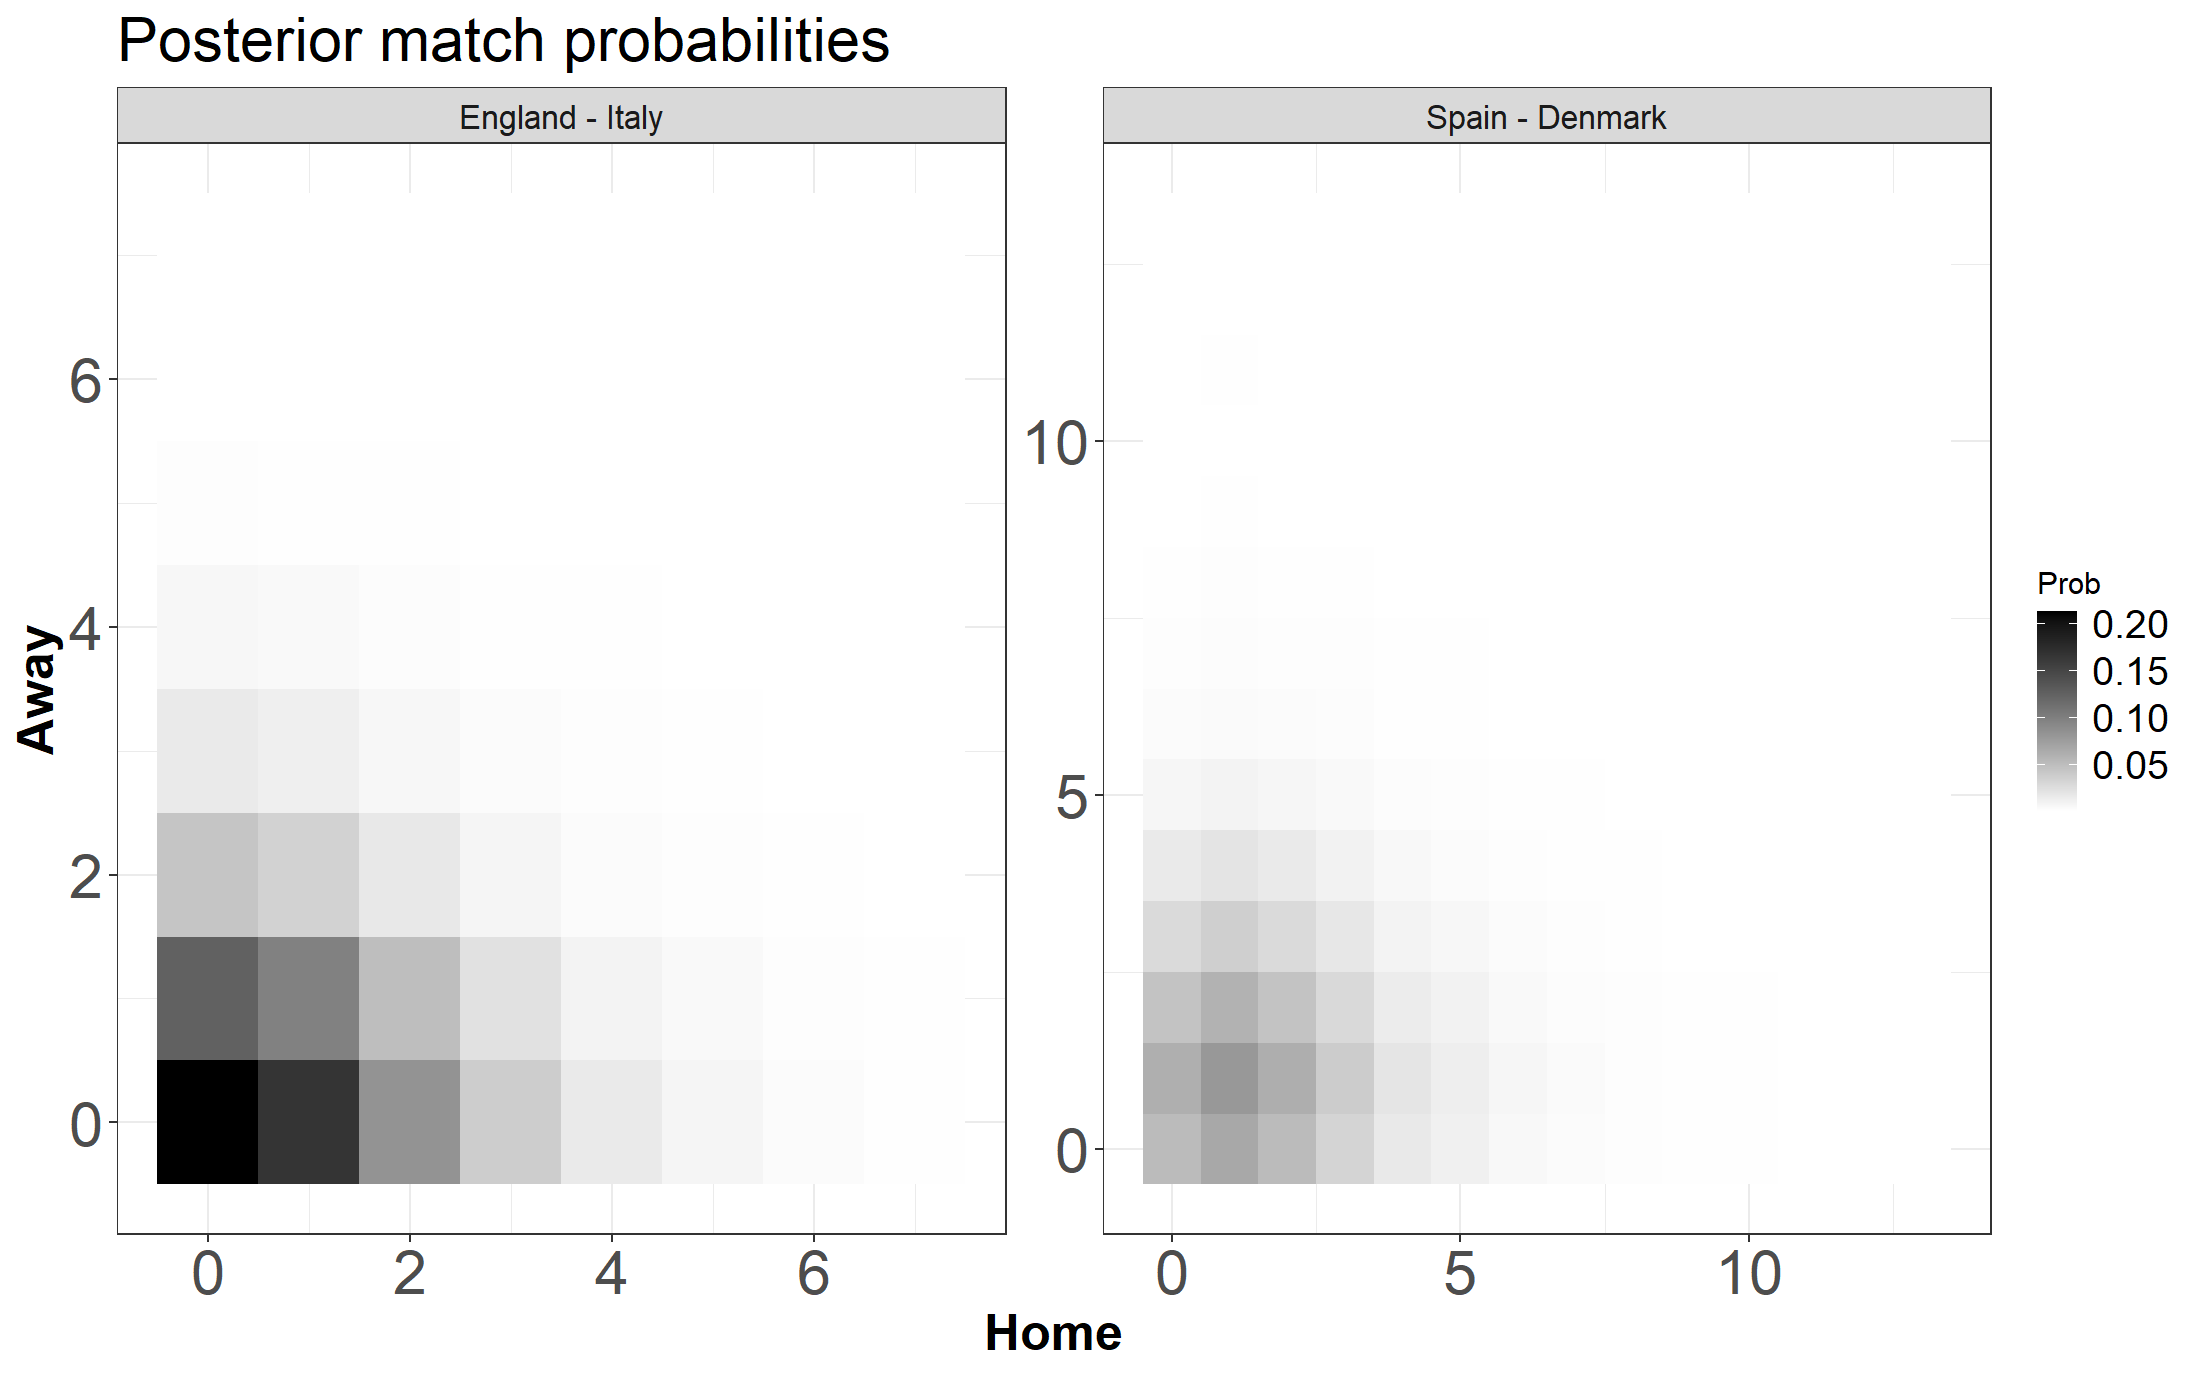
\includegraphics[width=0.8\linewidth]{figs/data2-1} \end{center}

\end{document}
